\chapter{\albatros~Experiment}

%Array of Long Baseline Antennas for Taking Radio Observations from the Sub-antarctic
    \section{Overview of the Pathfinder}
    \section{Pathfinder System Signal Chain}
	    \begin{figure}
	    	\begin{center} 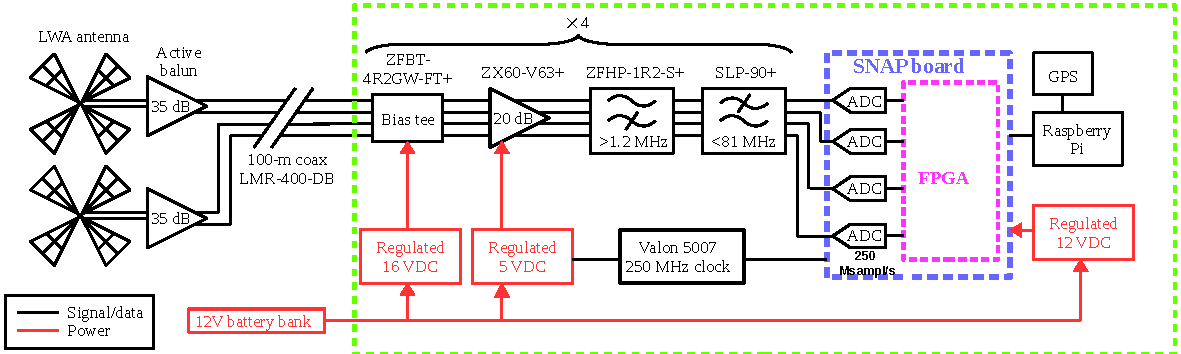
\includegraphics[width=\linewidth]{Figures/pathfinder_schematic.pdf}
	    		\caption{Two-element \albatros\ pathfinder block diagram.  Signals
	    			from two dual-polarzation LWA antennas are amplified by
	    			front-end active baluns~\citep{2012PASP..124.1090H}.  The
	    			antennas are connected via 100-m coaxial cables to the back-end readout electronics, which are housed in a Faraday cage denoted by the dashed box.  Each of the four antenna outputs is passed to a second-stage electronics chain consisting of filters and	further amplfication.  The signals are digitized at 250~Msamp/s by a SNAP board, which includes an on-board FPGA that computes
	    			auto- and cross-spectra from and between the four inputs.  A Raspberry Pi controls the SNAP board and saves the data.}
	    		\label{Fig:albatros2_schem}
	    	\end{center}
	    \end{figure}
   
        \subsection{}
        \subsection{}
        \subsection{}
        \subsection{}
        
        
\newpage
    \section{Overview of Autonomous Stations}
    \section{Autonomous Stations Signal Chain}
    
    \begin{figure}
    	\begin{center}
    		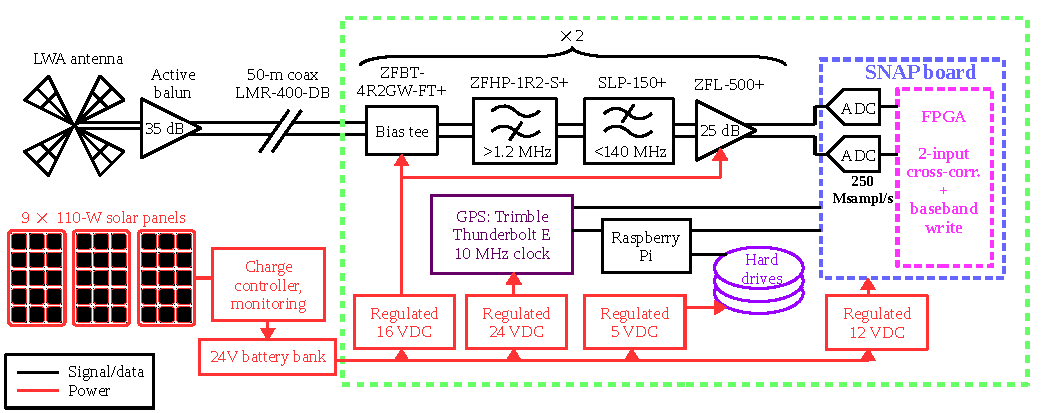
\includegraphics[width=\linewidth]{Figures/albatros_single_schematic.pdf}
    		\caption{Single-antenna autonomous station block diagram.  A dual-polarization LWA antenna, equipped with a front-end active balun, connects via 50-m coaxial cables to the back-end readout electronics, housed in a Faraday cage denoted by the dashed box. Each of the two antenna signals is passed to a second-stage	electronics chain consisting of filters and further amplfication.  The signals are digitized at 250~Msamp/s by a SNAP board, which includes an on-board FPGA that computes channelized baseband and spectra from both inputs.  A Raspberry Pi controls the SNAP board and receives the baseband data and spectra.  The baseband data are saved to external hard drives. The system is powered by solar panels that charge a 24-V battery	bank.}
    		\label{Fig:albatros1_schem}
    	\end{center}
    \end{figure}
    
        \subsection{}
        \subsection{}
